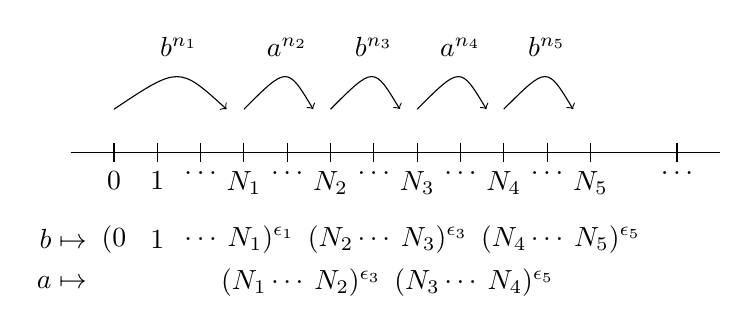
\begin{tikzpicture}[scale = 1.1]
\draw (-.5,0) -- (7,0) ;

\draw[shift={(0,0)},color=black] (0pt,3pt) -- (0pt,-3pt);
\draw[shift={(0,0)},color=black] (0pt,0pt) -- (0pt,-3pt) node[below] 
{$0$};
\draw[shift={(0.5,0)},color=black] (0pt,3pt) -- (0pt,-3pt);
\draw[shift={(0.5,0)},color=black] (0pt,0pt) -- (0pt,-3pt) node[below] 
{$1$};
\draw[shift={(1,0)},color=black] (0pt,3pt) -- (0pt,-3pt);
\draw[shift={(1,0)},color=black] (0pt,0pt) -- (0pt,-3pt) node[below] 
{$\dots$};
\draw[shift={(1.5,0)},color=black] (0pt,3pt) -- (0pt,-3pt);
\draw[shift={(1.5,0)},color=black] (0pt,0pt) -- (0pt,-3pt) node[below] 
{$N_1$};
\draw[shift={(2,0)},color=black] (0pt,3pt) -- (0pt,-3pt);
\draw[shift={(2,0)},color=black] (0pt,0pt) -- (0pt,-3pt) node[below] 
{$\dots$};
\draw[shift={(2.5,0)},color=black] (0pt,3pt) -- (0pt,-3pt);
\draw[shift={(2.5,0)},color=black] (0pt,0pt) -- (0pt,-3pt) node[below] 
{$N_2$};
\draw[shift={(3,0)},color=black] (0pt,3pt) -- (0pt,-3pt);
\draw[shift={(3,0)},color=black] (0pt,0pt) -- (0pt,-3pt) node[below] 
{$\dots$};
\draw[shift={(3.5,0)},color=black] (0pt,3pt) -- (0pt,-3pt);
\draw[shift={(3.5,0)},color=black] (0pt,0pt) -- (0pt,-3pt) node[below] 
{$N_3$};
\draw[shift={(4,0)},color=black] (0pt,3pt) -- (0pt,-3pt);
\draw[shift={(4,0)},color=black] (0pt,0pt) -- (0pt,-3pt) node[below] 
{$\dots$};
\draw[shift={(4.5,0)},color=black] (0pt,3pt) -- (0pt,-3pt);
\draw[shift={(4.5,0)},color=black] (0pt,0pt) -- (0pt,-3pt) node[below] 
{$N_4$};
\draw[shift={(5,0)},color=black] (0pt,3pt) -- (0pt,-3pt);
\draw[shift={(5,0)},color=black] (0pt,0pt) -- (0pt,-3pt) node[below] 
{$\dots$};
\draw[shift={(5.5,0)},color=black] (0pt,3pt) -- (0pt,-3pt);
\draw[shift={(5.5,0)},color=black] (0pt,0pt) -- (0pt,-3pt) node[below] 
{$N_5$};
\draw[shift={(6.5,0)},color=black] (0pt,3pt) -- (0pt,-3pt);
\draw[shift={(6.5,0)},color=black] (0pt,0pt) -- (0pt,-3pt) node[below] 
{$\dots$};

\draw[->] (0, .5) .. controls (.75,1) .. (1.3, .5);
\draw[->] (1.5, .5) .. controls (2,1) .. (2.3, .5);
\draw[->] (2.5, .5) .. controls (3,1) .. (3.3, .5);
\draw[->] (3.5, .5) .. controls (4,1) .. (4.3, .5);
\draw[->] (4.5, .5) .. controls (5,1) .. (5.3, .5);

\node[above] at (.75, 1) {$b^{n_1}$};
\node[above] at (2, 1) {$a^{n_2}$};
\node[above] at (3, 1) {$b^{n_3}$};
\node[above] at (4, 1) {$a^{n_4}$};
\node[above] at (5, 1) {$b^{n_5}$};

\node[left] at (-.2, -1) {$b \mapsto $};
\node[left] at (-.2, -1.5) {$a \mapsto $};

\node at (0, -1) {$(0$};
\node at (0.5, -1) {$1$};
\node at (1, -1) {$\dots$};
\node[right] at (1.2, -1) {$N_1)^{\epsilon_1}$};

\node at (2.5, -1) {$(N_2$};
\node at (3, -1) {$\dots$};
\node[right] at (3.2, -1) {$N_3)^{\epsilon_3}$};

\node at (4.5, -1) {$(N_4$};
\node at (5, -1) {$\dots$};
\node[right] at (5.2, -1) {$N_5)^{\epsilon_5}$};

\node at (1.5, -1.5) {$(N_1$};
\node at (2, -1.5) {$\dots$};
\node[right] at (2.2, -1.5) {$N_2)^{\epsilon_3}$};

\node at (3.5, -1.5) {$(N_3$};
\node at (4, -1.5) {$\dots$};
\node[right] at (4.2, -1.5) {$N_4)^{\epsilon_5}$};

\end{tikzpicture}

